%!TEX root = thesis.tex

\chapter{Introduction}
\par
Creating detailed virtual worlds can be a tedious task for artists. Indeed, modelling terrain, vegetation, rivers, water reserves, soil, rocks, buildings and road networks for large virtual worlds manually can be extremely burdensome. This is especially true when realism is a key requirement. The increase in size and complexity of these virtual worlds mirror that of the processing capabilities of computing hardware. As a consequence, the task is only becoming more time consuming.\\

A popular technique that overcomes the burden of repetitive tasks is to have them automated. This involves algorithms which, given a set of input parameters, generate the required content automatically. This is called \textit{procedural content generation} and has been successfully applied in different areas of computer graphics, including: the generation of non-repetitive textures \cite{Efros1999,Liang2001,Wei2009}, modelling plants \cite{Boudon2012,Fourcaud2008,Guo2011,Lewis1999}, creating terrains \cite{Smelik2009,Gain2009,Doran2010}, generating river networks \cite{Derzapf2011,Emilien} and producing city landscapes \cite{Gain,Kelly2007,Parish2001} (figure \ref{fig:procedrual_generated_content_examples}) \\
A common difficulty with these methods, however, is finding the appropriate input parameters for the procedural algorithms. The correlation between the parameters and the resulting content is often unintuitive and, as a consequence, often requires iterative trial-and-error until a sufficiently acceptable result is found. To overcome this, interactive techniques are often used in an attempt to make generating the input parameters more intuitive. These range from simple paint tools such as lassos and brushes \cite{Emilien} to sketch-based algorithms \cite{Gain2009}. \\

\begin{figure}[h]
  \centering
	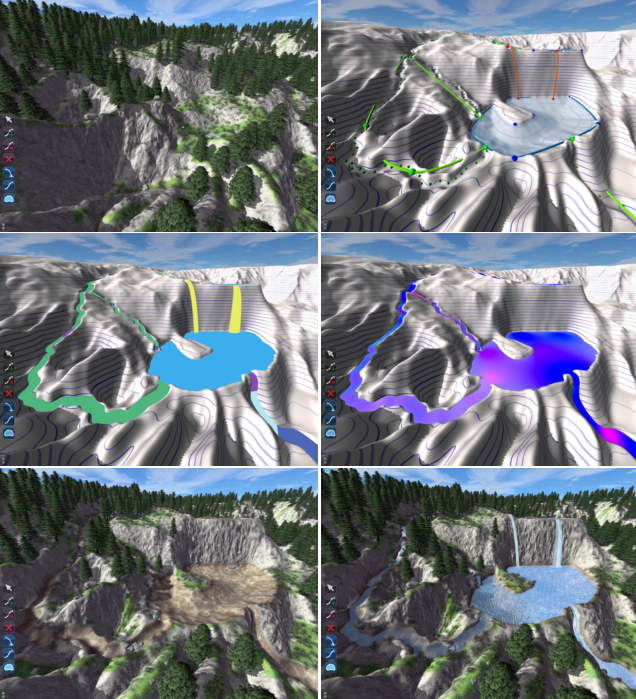
\includegraphics[width=\textwidth]{procedurally_generated_content_example.png}
	\caption{\textit{Example of a scene with procedurally generated terrain, vegetation and water networks \cite{Emilien2014a} }}
	\label{fig:procedrual_generated_content_examples}
\end{figure}

The intent of this thesis is to develop procedural algorithms to automate the generation of virtual rural worlds. More specifically, this work focuses on procedurally generating two core properties of rural worlds: vegetation and water networks. The input parameters for the procedural algorithms developed must be interactive or self-explanatory. 

\newpage
\section{Research Goals}

This research aims to answer whether or not procedural algorithms can be developed to automate the generation of realistic vegetation and water networks for virtual worlds. It also tries to answer if making these algorithms configurable permits the generation of a wide spectrum of virtual worlds. Finally, by optimizing the core algorithms, we will explore whether real-time interactions can be achieved. \\

Rephrased as research goals, this work attempts to:
\begin{itemize}
\item Develop procedural methods to automate the generation of realistic virtual rural worlds.
\item When possible, provide real-time interaction.
\end{itemize}

One of the most important aspect of rural landscapes is vegetation. As such, our \textit{first goal} must strongly focus on the placement of plants. The automation provided should not limit user control and the flexibility of the system. For example, it must be possible to generate worlds with varying elevations, river networks, water sources and vegetation. To test whether this is achieved, vegetation is generated and analysed for different virtual worlds varying in resource availability. The resulting vegetation is then analysed to ensure validity and plausibility. \\

Generating realistic water networks is also a key requirements of our \textit{first goal}. The rivers should follow natural erosion lines and their appearance should be correlated to configured rainfall. To test the validity of the water network generation algorithm, terrains representing given locations on earth are loaded, water networks procedurally generated and compared with the real world equivalent. \\

Maintaining a continuous feedback loop between user action and corresponding reaction is extremely important for both user-friendliness and to optimize usage. In an attempt to meet our \textit{second goal}, therefore, efficient algorithms must be developed in order to keep time complexity to a minimum. When suited, these algorithms should be developed to run on the GPU. To test this, the processing time of each component is analysed in detail to deduce algorithmic complexity along with the procedural parameters which bare a strong influence. \\

\section{Contributions}

The primary contributions of this thesis are:
\begin{itemize}
\item A carefully designed interface permitting users to model any environment with minimal effort.
\item An efficient procedural water network generation algorithm, which relies solely on soil, rainfall and terrain properties.
\item A novel vegetation generation component, which uses clustering, statistical analysis and a simulator to ensure both realism and efficiency.
\end{itemize}

\section{Structure}

To start, a detailed overview of existing work is presented in chapter \ref{chap:background}. To better understand the individual system components of this work, an overview of the system is given first in chapter \ref{chap:system_overview}. Chapter \ref{chap:terrain_and_resources} outlines how the base terrain is specified, associated resources configured and water content procedurally generated. The clustering algorithm used to group vertices based on associated resources is discussed and its performance analysed in chapter \ref{chap:clustering}. Chapter \ref{chap:vegetation} discusses the techniques used to deduce suitable vegetation and efficiently generate highly detailed and large scale plant distributions. Test environments are generated and the systems strengths and weaknesses discussed in chapter \ref{chap:results}. Finally, in chapter \ref{chap:conclusion}, the thesis is concluded and future directions explored.
